\documentclass[CS4204-Notes.tex]{subfiles}
\begin{document}

\section{Introduction}
Parallel programming is about programming on multicore/manycore machines. There are generally two forms of parallel programming, low level parallelism with pThreads, OpenMP, CUDA etc and higher level parallelism with function languages such as Haskell. 
\n
In the past, the performance of consumer processors was improved from increased clock speed as transistors grew smaller. However as we are reaching the limits of improvements to silicon and hardware technology, consumer processors have started to take the direction of focusing on parallel architectures with multicore systems. Purely functional languages are beneficial for programming parallel systems thanks to the absence of side effects, making it easy to evaluate sub-expressions in parallel. The only issue is the trivial work required to evaluate sub-expressions is not out balanced by the overhead needed to spawn a parallel thread to deal with it. 

\subsection{What is Multicore?}
Multicore architectures refer to having more than one processor on a single computer chip, where a processor is defined as a logical processing unit rather than a physical one. For example Intel's hyperthreading allows a single processor to act as two virtual processors. Multicore architectures also share many resources as a result of being on the same chip:
\begin{itemize}
\item Shared memory
\item Shared address space
\item Shared data bus
\item \textit{Independent} instruction streams
\item Shared cache
\end{itemize}
The increased amount of shared resources, such as the shared bus and shared memory and cache leads to more contention as all processors compete for resources. Multicore architectures are important in today's technological advances, not just in consumer desktop machines and mobile devices. In particular, grid/cloud computing systems, embedded systems, IoT and SIMD/MIMD architectures and GPUs all take advantage of parallel computation. 

\subsubsection{Manycore and megacore}
In the future, it may be likely that rather than the current multicore chips, the number of processors start scaling to many/megacores with hundred or thousands of processors on a single chip. These \textit{manycore} machines are likely to have more, individually less-powerful processors and may communicate through some kind of communication network rather than a shared bus.
\begin{figure}[H]
\centering
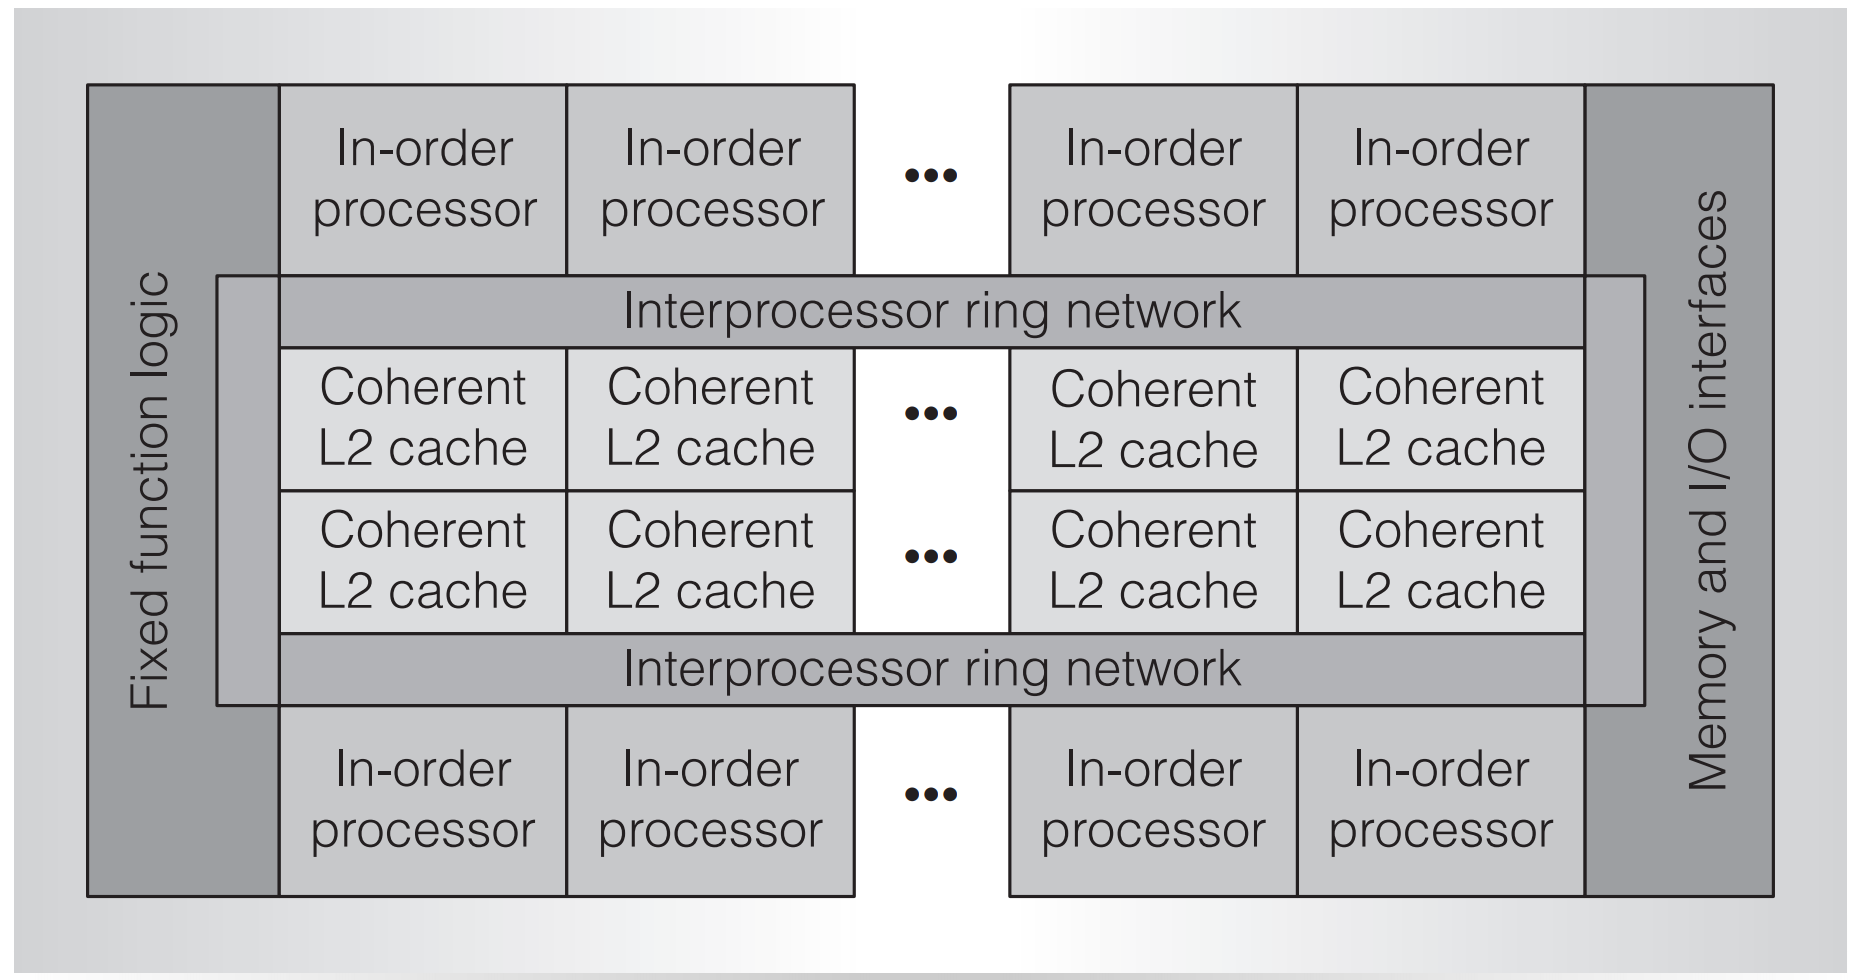
\includegraphics[width=0.8\textwidth, keepaspectratio]{imgs/manycore-architecture.png}
\caption{Schematic of the Larrabee manycore architecture.}
\end{figure}
\noindent
In these many/megacore architectures, it is likely to not simply be a scaled version of today's multicore chips with more cores. As there can be many processors, there could be hundreds of dedicated but lightweight units with \textit{few} heavyweight general purpose processors. It is also likely there would be specialised units for specific functions, such as RSA encryption or network protocols. This leads to a highly \textbf{heterogeneous processor} which is combination of many specialised units. Furthermore, this will likely \textit{not} have shared memory, having a NUMA (Non-Uniform Memory Access) design instead. 

\subsection{Concurrency vs Parallelism}
\textbf{Concurrency} is the concept that more than one thread may be executing simultaneously. Depending on the implementation, concurrent threads may execute in parallel or sequentially. Concurrency is generally used to identify logically-independent units of computation (no dependencies), for example in a user interface, which often yields relatively small-scale parallelism.
\n
\textbf{Parallelism} on the other hand is the idea of executing more than one thread simultaneously on separate hardware devices. This is usually done for performance reasons, as opposed to concurrency, which is introduced for structural reasons so that independent threads can be assigned to different program elements. 

\subsection{Challenges of parallel programming}
As the future of multicore chips moves in a more heterogeneous direction, there is a need for programs to be developed in an integrated way. It will be impossible to program each core differently and take static decisions about placement. Moreover, issues of time, energy, security etc. have to be taken into account in the design. The challenge is to think and program in a parallel way that is not the same as writing concurrent code. 
\begin{displayquote}
\textit{Ultimately, developers should start thinking about} tens, hundreds and thousands \textit{of cores} now \textit{in their algorithmic development and deployment pipeline}
\n
\textbf{Anwar Ghuloum, Principal Engineer, Intel Microprocessor Technology Lab}
\end{displayquote}
A large issue is that it is non-trivial to transform sequential code into parallel programs. In fact, many applications will actually \textit{run slower}, especially for larger systems. Up to 2-8 or even 16 cores, it is possible to simply write modified sequential code and use multiple programs to keep processors busy, but a much larger and complicated change is required for larger systems. 
\n
The typical approach of writing concurrent code is \textbf{not} the same as parallelism. Concurrency is all about breaking down programs into independent units of computation while parallelism is about making things happen at the same time. In many cases of concurrent programming, the programs are developed at a low level of abstraction without first understanding the parallelism. The issues this brings is concurrent programs which are designed with specific architectures in mind rather than with general parallel abstractions and structure. Furthermore, concurrency only gives an \textit{illusion} of independent threads of execution with a few \textbf{huge} threads, while parallelism is about the \textit{reality} of threads executing at the same time with thousands or millions of \textbf{tiny} threads.
\n
Concurrency must also deal with maintaining dependencies, as units of execution must be kept in order with dependencies to remain correct. The point of parallelism is to break dependencies. 

\subsubsection{Divide and conquer}
The divide and conquer pattern is a simple example of parallelism where the problem only solves the program at the trivial case, otherwise it is continually divided into two or more parts, with each solved independently and the results combined. 
\begin{figure}[H]
\centering
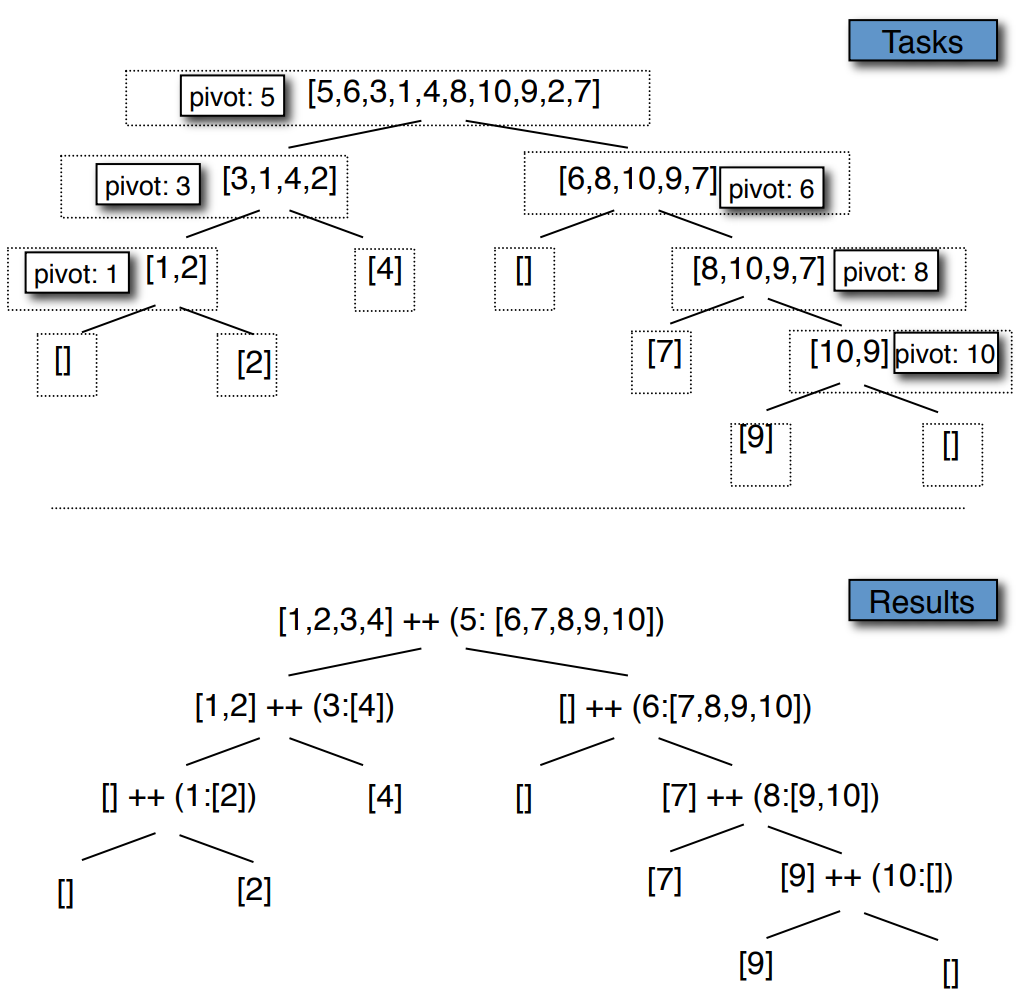
\includegraphics[width=1\textwidth, keepaspectratio]{imgs/divide-and-conquer.png}
\caption{Quicksort using divide and conquer to the trivial case of one element.}
\end{figure}
\noindent
To implement this divide and conquer algorithm with pThreads, threads have to be created and joined for each left and right of the split. This leads to too much complexity to manage and makes it difficult to scale unless the program is simple. There are issues with deadlocks, race conditions, non-determinism and communication that have to be dealt with by the systems programmer, which ideally should be abstracted away from an application programmer. Fundamentally, this means programmers must learn to think in parallel, which requires new high level constructs. 

\end{document}